% ---------------------------------------------------
% ----- Chapters of the template
% ----- for Bachelor-, Master thesis and class papers
% ---------------------------------------------------
%  Created by C. Müller-Birn on 2012-08-17, CC-BY-SA 3.0.
%  Freie Universität Berlin, Institute of Computer Science, Human Centered Computing. 
%
\chapter{Hintergrund der Arbeit}
\label{chap:background}

	\section{Definition nichttechnische Experten}
	Da die im Rahmen dieser Arbeit entwickelte Software für die Nutzung von
	nichttechnischen Experten vorgesehen ist, ist es sinnvoll diese zu definieren.
	Im Kontext dieser Arbeit sind damit Personen gemeint, die in den meisten Fällen
	beruflich mit Ontologien interagieren, in denen Konzepte ihrer Disziplin oder
	Domäne behandelt werden. Diese Personen haben aber keinen Hintergrund in der
	Informatik oder verwandten Fachgebieten. Aufgrund dessen haben sie begrenztes
	Wissen über die Vorgänge in Software und eine andere Sicht auf Software, als
	Personen mit technischem Hintergrund. In ihrer Arbeitsumgebung haben sie oft
	keine erweiterten Recht, um z.B. Software eigenständig zu installieren.

	\section{Mapping Methoden}
	Der grundlegende Prozess für die Bestimmung möglicher Matches von Eigenschaften
	sieht wie in Abbildung \ref{fig1} gezeigt aus. Das zentrale Element dabei ist
	der oder die Matcher. \cite{Hoo14}
	
	\begin{figure}[ht]
	\centering
	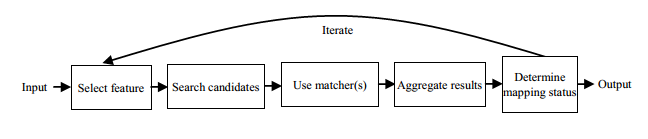
\includegraphics[width=1.0\textwidth]{pics/simple-high-level-view-of-a-mapping-process.png}
	\caption{Eine einfache Übersicht des Mapping Prozesses Nach \cite{Hoo14}}
	\label{fig1}
	\end{figure}
	
	Im ersten Schritt wird ein Element (\textit{feature}), wie ein Label für
	Entitäten oder Instanzen von Attributen, aus einer der zu matchenden Ontologien ausgewählt,
	anschließend werden in der anderen Ontologie nach möglichen, passenden
	Elementen (sogenannte \textit{candidates}) gesucht. Mithilfe der Matcher werden
	die beiden Eigenschaften dann verbunden, sofern der oder die Matcher Übereinstimmungen vermuten. Die Ergebnisse werden dann zusammengefasst und zum Schluss entweder in einer neuen Iteration berücksichtigt oder ausgegeben. \cite{Hoo14}\\
	Neben der direkten Verbindung kann man die Eigenschaften aus den Ontologien, die
	gematched werden sollen, über sogenannte \textit{Anker} (Anchors) mit einer
	weiteren Ontologie verbunden, deren Zweck es ist, als „Meta-Ontologie“ eine gemeinsame Schnittstelle zu bilden. Anker sind Entitäten, die als gleichartig zu Entitäten der anderen Ontologien definiert werden. \cite{Hoo14}
	
	\section{Kategorien von Matchern}
	\label{MatcherKategorien}
	Um Ontologien zu matchen gibt es verschiedene Möglichkeiten. Diese können einzeln, aber auch kombiniert auf verschiedene Weise angewendet werden. Eine Möglichkeit ist es, mehrere Matcher sequentiell anzuwenden, um die Ergebnisse immer mehr zu verfeinern und zu verbessern. Eine andere Variante ist es, mehr als eine Matching Methode parallel anzuwenden und dann die Ergebnisse zusammenzufügen. Diese beiden Aggregationsverfahren kann man auch kombinieren. \cite{Hoo14}
	
	\section{Terminologisches Mapping}
	Um Elemente von Ontologien zu matchen, kann man deren Benennung durch Tokenisierung in ein gemeinsames Format überführen und dann mithilfe von Gewichtung und Gleichheit in Relation setzen.
	\begin{itemize}
		\item Stringbasiert: Bei dieser Methode wird die Struktur von Strings als
		Zeichenketten betrachtet. Konkret werden Techniken angewendet, die Ähnlichkeit von Strings und deren Teilen bestimmen. Bekannte Methoden aus diesem Bereich sind z.B. Normalisierung und Editierdistanz. \cite{EuzShv07}  Beispielsweise beträgt der Abstand der Elemente „author“ und „hasauthor“ 3, nämlich den Zusatz „has“, sofern der Algorithmus erkennt, dass der hintere Teil gleich ist.
		\item  Sprache basiert: Hierbei werden Wörter als Texte betrachtet, d.h. die
		Reihenfolge der Wörter in einer Sequenz wird einbezogen, ebenso die Bedeutung dieser Wörter. Zur Analyse werden verschiedene Techniken angewandt, um das Grundwort zu ermitteln. Dieses dient dann dazu, Ähnlichkeiten zwischen den Wörtern zu finden. \cite{EuzShv07}  Zum Beispiel, wenn man in einer Ontologie das Element „walk“ und in einer anderen „walking“ hat, kann man „walking“ auf „walk“ reduzieren (z.B. durch Stemming) und dadurch Matches finden.
		\item Linguistische Analyse: Durch das Einbeziehen von externen
		linguistischen Quellen, wie z.B. Wiktionary , werden Strings interpretiert.
		Beim bedeutungsbasierten Ansatz werden über \textit{Hyponyme} (begriffliche
		Unterordnung), \textit{Hyperonyme} (Ober-/Überbegriff), \textit{Synonyme}
		(gleiche Bedeutung) und \textit{Antonyme} (gegensätzliche Bedeutung) die
		Bedeutung der Wörter festgestellt. Beim sprachbasierten Ansatz hingegen, wird der Abstand zu anderen Wörtern in Sätzen analysiert. \cite{EuzShv07} Zum Beispiel kann man „creator“ als Oberbegriff von „author“ und „illustrator“ auffassen.
	\end{itemize}
	
	\section{Strukturelles Mapping}
	\label{StrukturellesMapping}
	Eine zweite Möglichkeit für das Matching von Ontologien ist das Betrachten der Strukturen innerhalb der Ontologien. Dabei werden die Eigenschaften und die Beziehung der Entitäten untereinander untersucht.
	\begin{itemize}
		\item Taxonomisches Mapping: Dabei werden zwei Techniken verwendet,
		\textit{super-} oder  \textit{subclass rule} und \textit{bounded-paths}. Die
		\textit{super class rule} unterstellt, dass eine Ähnlichkeit zwischen zwei
		Konzepten besteht, wenn diese ein Elternkonzept teilen. \cite{EuzShv07}  Beispielsweise kann man annehmen, dass wenn zwei Ontologien ein gleiches oder ähnliches Konzept haben, um Bücher zu beschreiben, dass die darunterliegenden Konzepte für die Beschreibung für „creator“ und „author“ ebenfalls ähnlich bzw. gleich sind. Bei bounded-paths werden Pfade verglichen, um ähnliche Konzepte zu identifizieren. Bei diesen Pfaden handelt es sich um Verbindungen zwischen Klassen. Die Art und Weise der Verbindungen wird durch eine hierarchische Struktur definiert. \cite{EuzShv07} Wenn das Attribut „book“ in zwei verschiedenen Ontologien einmal mit „hasAuthor“ und einmal mit „hasWritten“ zu den beiden äquivalenten Elementen „creator“ bzw. „author“ verbunden ist, dann bieten sich diese beiden für eine Betrachtung bezüglich eines Matches an.
		\item Baumbasiertes Mapping: Hierbei spielt Ähnlichkeit eine Rolle. Es wird
		angenommen, dass sich Knoten ähneln, die benachbart sind, und dass dies auch für verschiedene Ontologien gilt. Also wenn ein Knoten mit einem anderen benachbart ist und mit einem Knoten aus einer anderen Ontologie verbunden ist, dann ähneln sich die benachbarten Knoten mit den beiden verbundenen. Wenn beispielsweise in einer Ontologie das Element „book“ über „author“ mit „human“ verbunden ist und in einer zweiten Ontologie „volume“ über „author“ mit „writer“, wobei festgelegt wurde, dass sowohl „book“ und „volume“, als auch die beiden „author“ Elemente äquivalent sind, besteht Grund zur Annahme, dass „human“ und „writer“ ebenfalls ähnlich sind.\cite{EuzShv07} 
	\end{itemize}
	
	\section{Recommender Systems}
	Als Recommender Systeme werden Software und Techniken bezeichnet, die dazu
	dienen, ihren Anwendern sinnvolle Vorschläge bezüglich Entscheidungen zu machen. Meist sind diese Systeme darauf hin ausgerichtet, unerfahrene oder nicht sachkundige Nutzer zu unterstützen. \cite{Fra10}  Bekannt sind den meisten Menschen solche System überwiegend aus den Bereichen des eCommerce, wo sie genutzt werden, um Kunden oder Besuchern Produkte vorzuschlagen, die diese interessieren könnten.\\
	In ihrer einfachsten Form, werden möglich Vorschläge in einer Liste gesammelt und dann entsprechend der Präferenzen des Nutzers und (Rand-)Bedingungen geordnet. Beide ergeben sich direkt, z.B. beim Ansehen eines Produkts in einem Webshop, oder indirekt, z.B. über die Empfehlung eines Films des gleichen Regisseurs. \cite{Fra10} 
	
	\section{Information Visualization}
	Bei der Information Visualization geht es im Kern darum, Daten grafisch
	darzustellen. Dadurch ist es möglich, Daten anzuzeigen, um den
	Nutzer bzw. Betrachter nicht das Interesse verlieren zu lassen. Weiterhin ermöglichen eine gute Aufbereitung der Daten und ein
	gutes User Iterface (UI) ein leichteres Navigieren innerhalb dieser Daten und deren Verknüpfung.\\
	Dafür gibt es eine Reihe an Techniken, um dies zu bewerkstelligen. Die
	Visualisierung von Informationen ist eng verknüpft mit der \textit{visuellen
	Datenexploration} (visual data exploration).
	Bei der visuellen Datenexploration werden Daten visualisiert, um es Menschen zu
	ermöglichen, diese Daten zu durchdringen, Schlüsse aus ihnen zu ziehen und direkt mit den Daten zu interagieren. \cite{Kei02}\\ Die manuelle Exploration von Daten kann zum Generieren von Hypothesen auf Basis von Daten genutzt werden, zusätzlich zur Anwendung von automatisierten Techniken aus der Statistik oder Machine Learning. Da diese beiden Arten von Techniken nicht immer anwendbar sind, kann man trotzdem gute Ergebnisse bei der Auswertung erzielen. Insbesondere wenn es  sich um stark inhomogene oder stark verrauschte Daten handelt. Zusätzlich kann man Datenexploration oft auch dann durchführen, ohne tiefgreifendes Verständnis von komplexen  mathematischen oder statistischen Algorithmen oder Parametern zu haben.\cite{Kei02}
	
	\section{Precision und Recall}
	Precision und Recall sind im Bereich der Information Retrieval verbreitete
	Maßeinheiten. Dort beziehen sie sich auf Dokumente.
	Wenn sie im Bereich des Ontologie Matchings eingesetzt werden, werden anstatt Dokumente Matching Paare
	gemessen. In beiden Fällen
	werden die zu untersuchende Menge mit einer Referenzmenge
	verglichen.\cite{Euz07} Einfach ausgedrückt, wird die Precision folgendermaßen berechnet\\
	\( \frac{\text{True positves der gefundenen Ergebnisse}}{\text{True
	positves der gefundenen Ergebnisse + false positves der gefundenen Ergebnisse}} \)
	\\
	Dadurch wird die Korrektheit der Ermittlungsmethode ermittelt\cite{Euz07}.
	Der Recall er gibt sich aus\\
	\( \frac{\text{True positves der gefundenen
	Ergebnisse}}{\text{True positves der gefundenen Ergebnisse + True positves der
	nicht gefundenen Ergebnisse}} \)
	\\
	Das dient zur Ermittlung der Vollständigkeit.\cite{Euz07}
	
	\cleardoublepage
	\pagebreak[4] 